A inclina��o de uma rampa � calculada da seguinte maneira: para cada metro medido na horizontal, mede-se x cent�metros na vertical. Diz-se, nesse caso, que a rampa tem inclina��o de x\%, como no exemplo da figura: 

\begin{figure}[h]
\centering
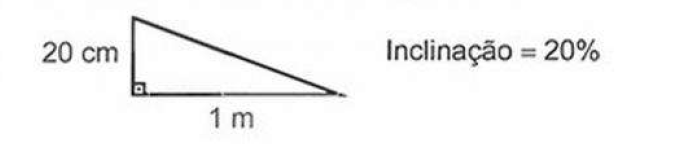
\includegraphics[width=8cm]{../figuras/q172(1)-2018.png}
\end{figure}

A figura apresenta um projeto de uma rampa de acesso a uma garagem residencial cuja base, situada 2 melros abaixo do n�vel da rua, tem 8 metros de comprimento. 

\begin{figure}[h]
\centering
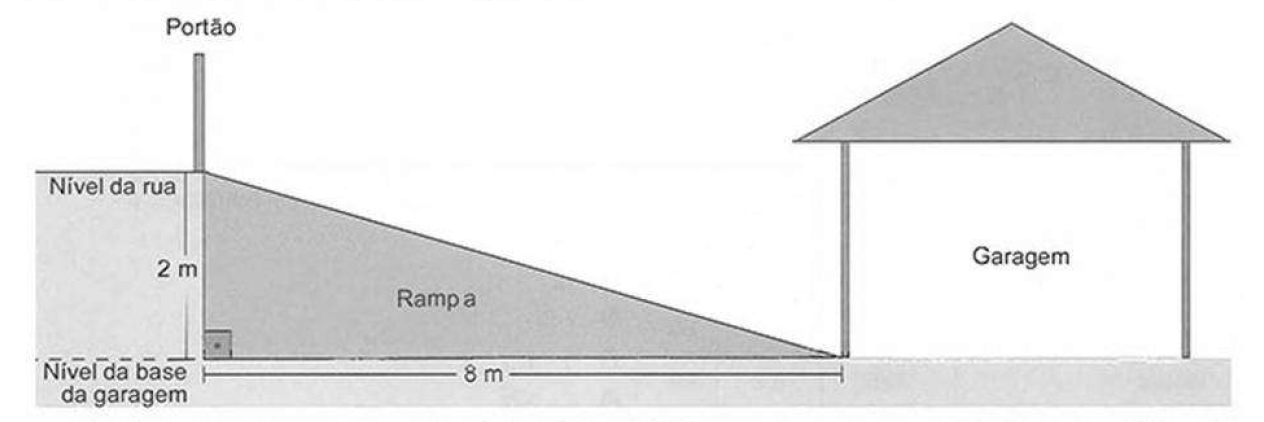
\includegraphics[width=8cm]{../figuras/q172(2)-2018.png}
\end{figure}

Depois de projetada a rampa, o respons�vel pela obra foi informado de que as normas t�cnicas do munic�pio onde ela est� localizada exigem que a inclina��o m�xima de uma rampa de acesso a uma garagem residencial seja de 20\%. 
Se a rampa projetada tiver inclina��o superior a 20\%, o n�vel da garagem dever� ser alterado para diminuir o percentual de inclina��o. mantendo o comprimento da base da rampa. 
Para atender �s normas t�cnicas do munic�pio, o n�vel da garagem dever� ser 

\begin{enumerate}
\item[a)]elevado em 40 cm
\item[b)] elevado em 50 cm 
\item[c)] mantido no mesmo n�vel
\item[d)] rebaixado em 40 cm 
\item[e)] rebaixado em 50 cm
\end{enumerate}